\section{Universal laws in RNA-Seq}
\subsection{TCGA}
Analysing TCGA dataset~\cite{grossman2016toward} the first interesting analysis is to plot the sorted abundance, this gives the so called Zipf's law. The analysis were made considering \textit{Gene Expression Quantification} as data type, \textit{Transcriptome Profiling} as data, \textit{RNA-Seq} as experimental strategy, \textit{HTSeq - Counts} or \textit{HTSeq - FPKM} as workflow type. $5000$ samples were downloaded and analysed.
\begin{figure}[htb!]
    \centering
    \begin{minipage}{0.45\textwidth}
    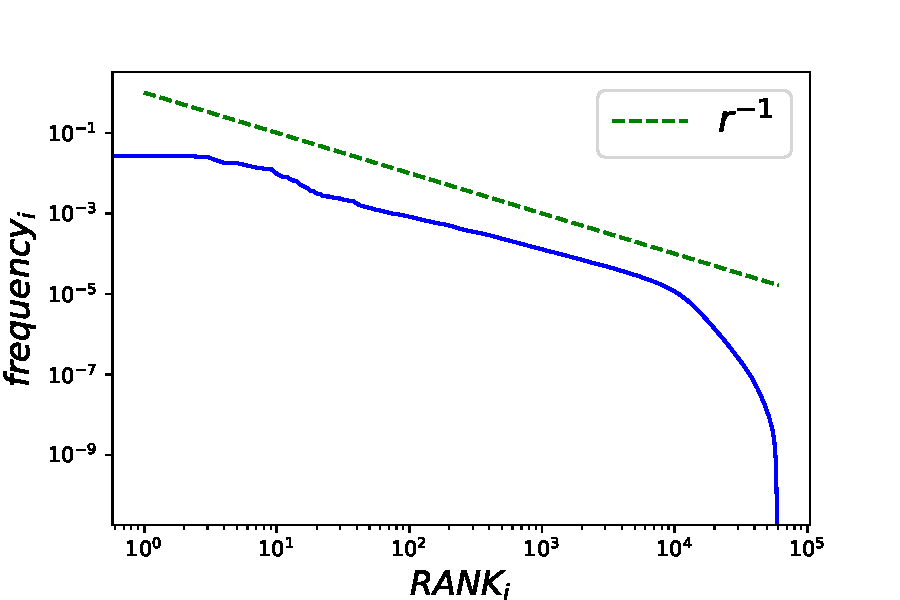
\includegraphics[width=0.95\linewidth]{pictures/structure/tcga/globalzipf_fpkmall.pdf}
    \end{minipage}
\hspace{3mm}
    \begin{minipage}{0.45\textwidth}
    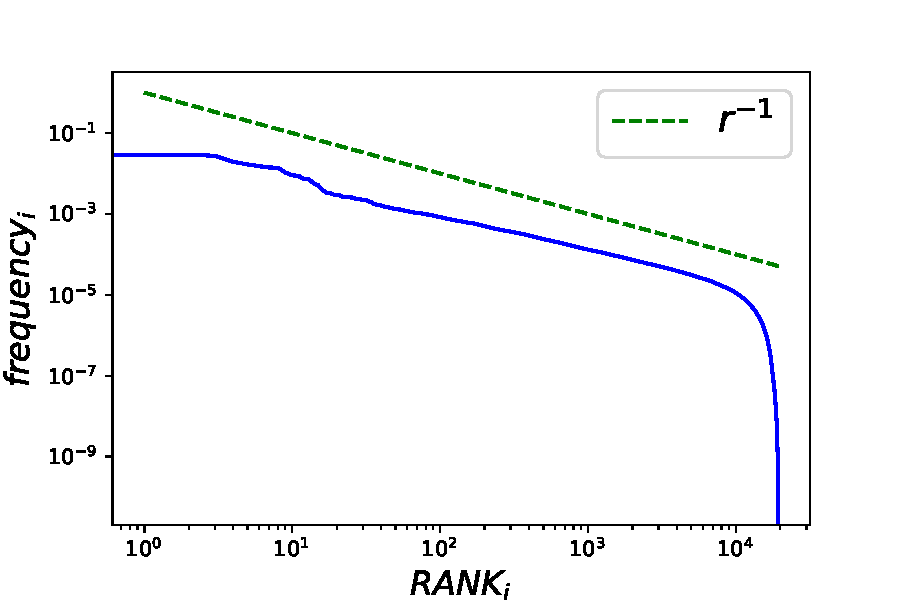
\includegraphics[width=0.95\linewidth]{pictures/structure/tcga/globalzipf_fpkm.pdf}
    \end{minipage}
    \caption{Zipf's law from FPKM normalised data. On the right considering only protein coding genes}
    \label{fig:structure/tcga/globalZipf}
\end{figure}
In figure~\ref{fig:structure/tcga/globalZipf} it is shown the frequency ranked plot. It is interesting that this kind of data distribute according a power law with exponent close to $1$, this same behaviour can be found in completely different systems such as linguistics' ones. Another interesting fact is that considering in the analysis also non-coding genes gives a double-scaled power law. This is due to the fact that non coding genes are also more specific and rare, so their frequencies are quite small compared to protein coding genes.

Changing normalisation and considering counts instead of FPKM, the result is quite similar. The power law is more flat, meaning that genes have more similar abundances in the whole dataset. 
\begin{figure}
    \centering
    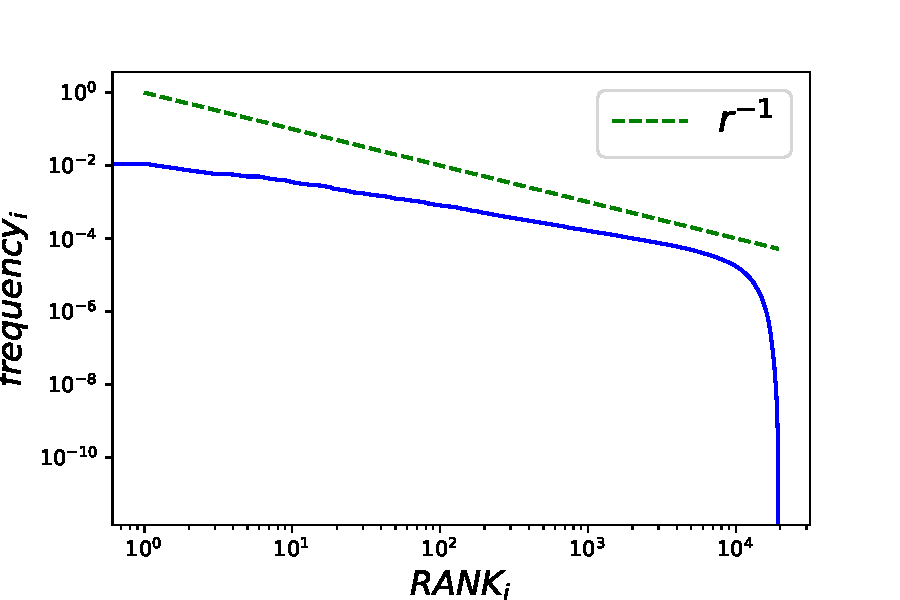
\includegraphics[width=0.8\linewidth]{pictures/structure/tcga/globalzipf_counts.pdf}
    \caption{Zipf's law of protein coding genes considering counts}
    \label{fig:structure/tcga/globalzipf_count}
\end{figure}

\subsection{GTEx}
A pretty similar analisys can be made on GTEx's~\cite{carithers2015novel} healthy samples. RNA sequencing raw counts data were download from file version \textit{2016-01-15 v7 RNASeQCv1.1.8}. All $\sim 11000$ samples available were considered at this time.

\begin{figure}[htb!]
    \centering
    \begin{minipage}{0.45\textwidth}
    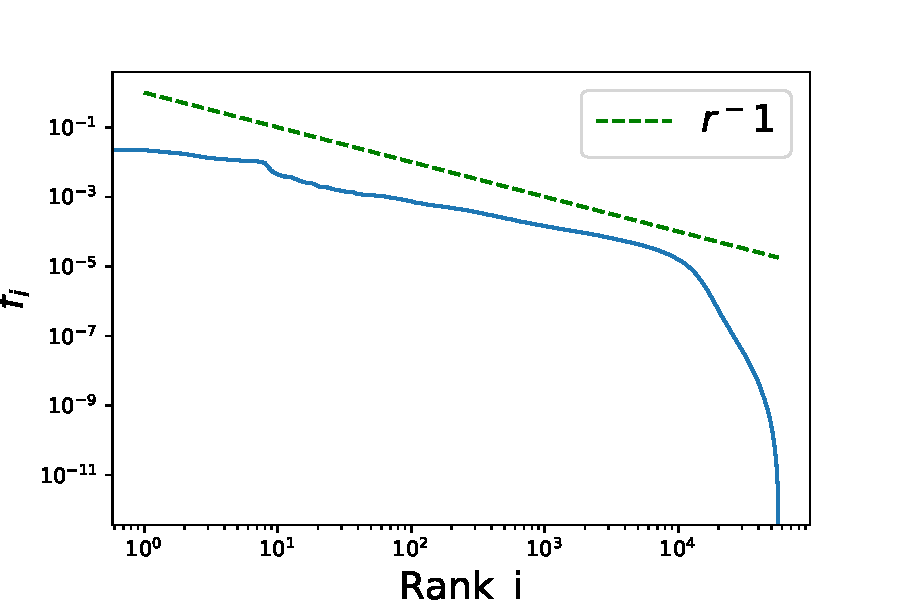
\includegraphics[width=0.95\linewidth]{pictures/structure/gtex/globalZipf.pdf}
    \end{minipage}
    \hspace{3mm}
    \begin{minipage}{0.45\textwidth}
    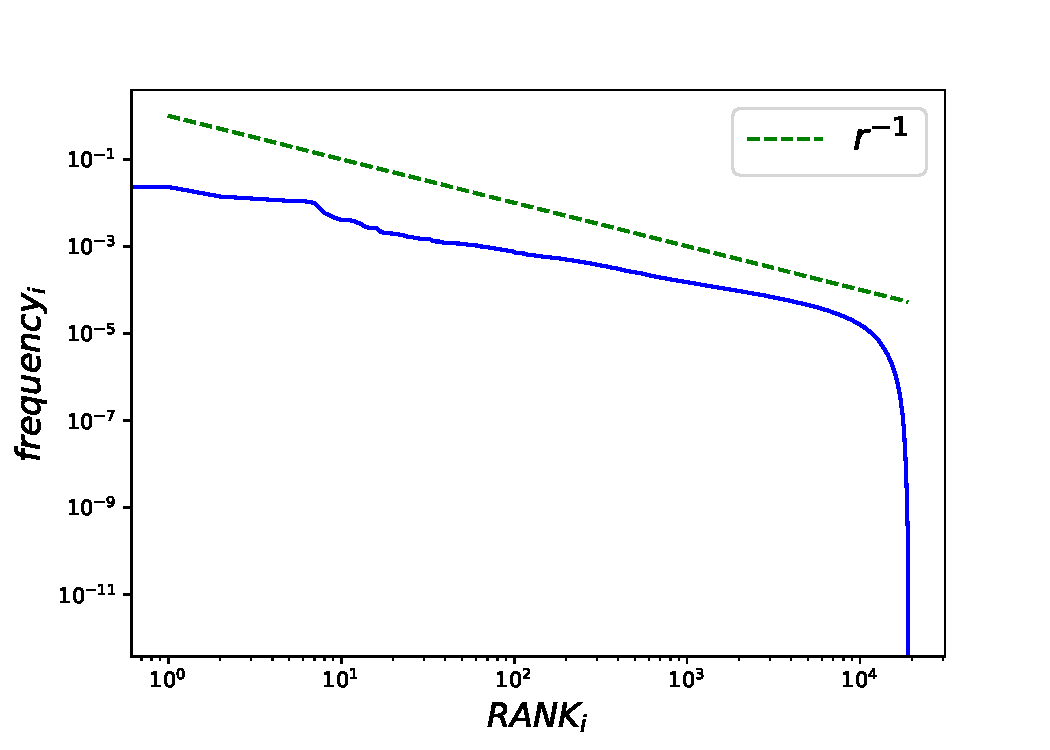
\includegraphics[width=0.95\linewidth]{pictures/structure/gtex/globalZipf_c.pdf}
    \end{minipage}
    \caption{Zipf's law from GTEx count data. On the left all genes considered, on the right only protein coding ones}
    \label{fig:my_label}
\end{figure}
Not surplisingly in the GTEx dataset it is retrieved the same beahviour at this time. The power law with exponent $\simeq 1$ is found and considering non coding genes gives to a knee in the power law.

Going further in the analysis it is possible make an histogram of occurrences defined by~\ref{eq:occurrence}, also known as $U$s.
\begin{figure}[htb!]
    \centering
    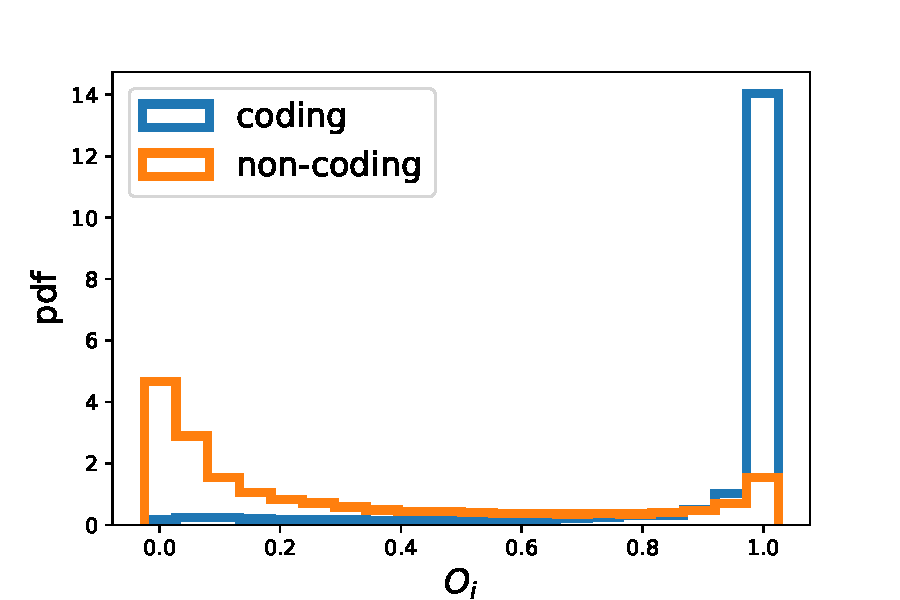
\includegraphics[width=0.9\linewidth]{pictures/structure/gtex/U_gtex_cnc.pdf}
    \caption{The histogram of the occurrences $O_i$}
    \label{fig:structure/gtex/U_cnc}
\end{figure}

Also in this kind of analysis it is possible to see the different behaviour of coding and not coding genes. The protein coding genes express almost in every sample, so their occurrence is near to $1$, non coding genes are more specific, so they are present only in a subset of the dataset and many of the have small occurrence.
\begin{figure}[htb!]
    \centering
    \begin{minipage}{0.45\textwidth}
    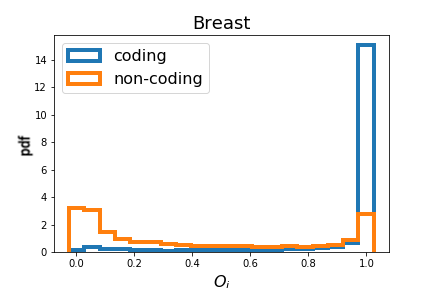
\includegraphics[width=0.95\linewidth]{pictures/structure/gtex/U_Breast.png}
    \end{minipage}
    \hspace{2mm}
    \begin{minipage}{0.45\textwidth}
    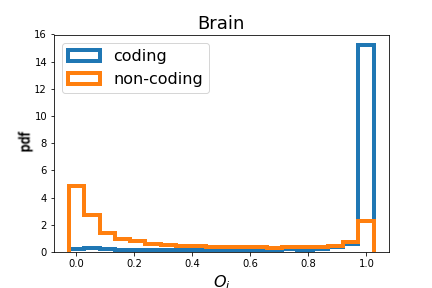
\includegraphics[width=0.95\linewidth]{pictures/structure/gtex/U_Brain.png}
    \end{minipage}
    \caption{Same behaviour is observed looking at one tissue a time.}
    \label{fig:structure/gtex/U_tissues}
\end{figure}
The same behaviour can be observed considering just all samples of a given tissue. In this case $O_i=0$ means that the genes has a non zero expression in just one of the samples of the tissue considered; in other words if a gene never express in a tissue it is not considered when constructing these tissue specific $U$ distributions.

From now on except were explicitly declared analysis will be made considering protein coding genes and counts with no normalisation.
